\documentclass{standalone}
\usepackage{pgfplots}
\pgfplotsset{compat=1.18}

\begin{document}
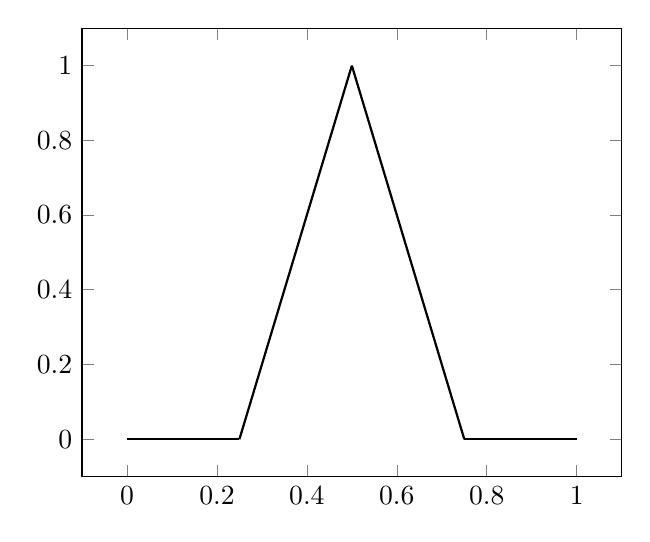
\begin{tikzpicture}[
    baseline, 
    declare function = {
      tent1(\x,\a,\h) = (\x-\a)/\h;
      tent2(\x,\a,\h) = (-\x+3*\a)/\h; 
    }
  ]
\begin{axis}[
xmin=-0.1,xmax=1.1,
ymin=-0.1,ymax=1.1,
]
\pgfmathsetmacro{\L}{1.0}
\pgfmathtruncatemacro{\Nsub}{4} 
\pgfmathsetmacro{\h}{\L/\Nsub} 
\typeout{check: h = \h}
\addplot [thick, domain=0:\h] {0};
\addplot [thick, domain=\h:2*\h] {tent1(x,\h,\h)};
\addplot [thick, domain=2*\h:3*\h] {tent2(x,\h,\h)};
\addplot [thick, domain=3*\h:4*\h] {0};

\end{axis}
\end{tikzpicture}
\end{document}